% !TEX encoding = UTF-8
% !TEX program = pdflatex
% !TEX root = InformationRetrieval.tex
% !TEX spellcheck = it-IT

% 17 Novembre 2016
%\chapter{Valutazione dei sistemi di reperimento}
%\section Il paradigma Cranfield

\section{Campagne di valutazione internazionali}

Sono delle iniziative internazionali che mira ad unire le risorse, umane e tecnologiche, di diversi gruppi di ricerca accademici e industriali necessarie per condurre la valutazione dei sistemi di IR.

Questo comprende la creazione di collezioni di test basate su esigenze reali, la condivisione dei risultati della valutazione dei sistemi e la discussione pubblica dei risultati ottenuti.

In questo modo è possibile confrontare diversi sistemi e metodi di reperimento dell'informazione in modo controllato, comparabile e ripetibile, nella speranza di accelerare il trasferimento di tecnologia verso il settore industriale.

Le principali campagne internazionali sono TREC, NTCIR, CLEF e FIRE.

\subsection{TREC}

Negli anni TREC ha prodotto varie collezioni di test ad-hoc che coprono diversi task (hanno obiettivi specifici), dalle collezioni generiche a quelle di solo brevetti o di immagini o di articoli di giornale, ecc.

Tipicamente le varie collezioni rilasciate da TREC sono composte da 500 a 750 mila componenti, per i quali sono definiti 50 topics. Per ogni topic vengono forniti: un \textit{titolo}, una descrizione ed una \textit{narrative} (una descrizione testuale estesa della query).

Con ogni collezione devono essere anche forniti anche i relativi giudizi di rilevanza, che specificano se un documento è rilevante o meno per il topic.
Considerando che TREC-1 ha 741856 documenti e 50 topic, si ha che i giudizi di rilevanza sono 37 milioni. Serve quindi un modo veloce per ottenerli.

\section{Creazione dei giudizi di rilevanza}

\begin{itemize}
	\item \textbf{Giudizi completi}: giudicare (\textit{assess}) ogni documento per ogni topic. Questo approccio è tipicamente impossibile o troppo oneroso, perché i giudizi devono essere dati da persone esperte riguardo il topic.
	\item \textbf{Campionamento casuale}: i giudizi vengono effettuati solo per dei campioni di documenti per ogni topic. C'è però un problema, perché per ogni topic devo avere un certo numero di documenti rilevanti, almeno 100, perché serve una base solida per determinare se un sistema funziona bene. Se c'è solo un documento rilevante su 600 mila non è possibile dare un giudizio corretto.
	\item \textbf{Campionamento basato sugli esperimenti (run)}: è il metodo adottato da TREC che viene detto anche \textbf{pooling}. Ovvero i campioni di documenti da giudicare vengono scelti con criterio, sfruttando il sistema di information retrieval per capire quali documenti sono più rilevanti.
	L'idea alla base è che se il sistema è fatto decentemente, riesce a trovare dei documenti rilevanti, creando un campione che quindi ne contiene un numero sufficiente.
	C'è poi da dire che il campione può essere generato accorpando i risultati di vari sistemi in modo da creare un pool migliore.
	Così facendo vengono limitati i costi.
	\`E ragionevole pensare che questo approccio crei un bias, perché se un sistema non viene preso in considerazione nella generazione del pool, i suoi documenti rilevanti non vengono presi in considerazione e magari quel sistema lasciato fuori è l'unico che recupera dei documenti particolarmente importanti.
	Tuttavia, generando i pool con un approccio leave-one-out è stato osservato che statisticamente questo bias non c'è.
	\item \textbf{Crowdsourcing}: chiedo aiuto a tante persone esterne, sottopagandole.
\end{itemize}

\subsection{run}

Definiamo $D = \{d_1, d_2, \ldots, d_n \}$ un'insieme di documenti e $T = \{ t_1, t_2, \ldots, t_m \}$ un insieme di topic con $m \ll n$.

Dato un numero naturale $N \in \mathbb{N}^+$ chiamato lunghezza della run, una \textbf{run} è definita come la funzione

\begin{align*}
R : T &\to D^N \\
	t &\to \mathbf{r}_t = (d_1, \ldots, d_N)
\end{align*}

\noindent tale che $\forall t \in T$, $\forall j,k \in [1,N] \ | \ j \neq k \Rightarrow \mathbf{r}_t[j] \neq  \mathbf{r}_t[k]$, dove $ \mathbf{r}_t[j]$ indica il $j$-esimo elemento del vettore.

Ovvero è una funzione che dato un topic $t \in T$ gli associa un sotto-insieme di documenti di cardinalità $N$ tale che tutti gli elementi del sotto-insieme siano distinti.

\begin{figure}[htbp]
	\centering
	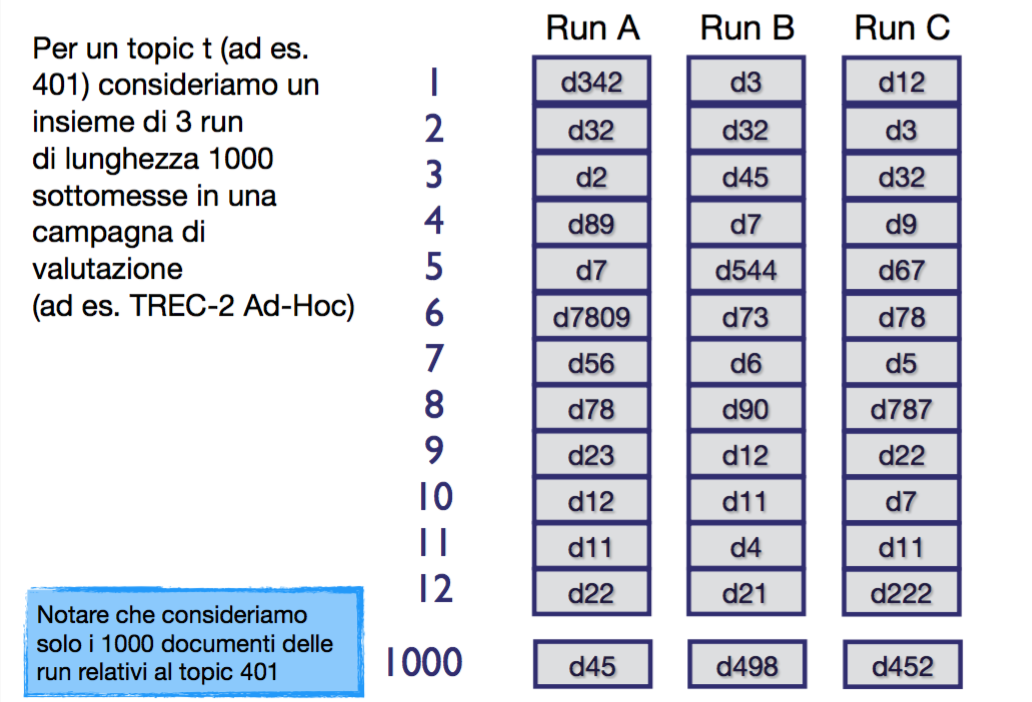
\includegraphics[width=0.5\textwidth]{images/l14-fig-1.png}
	\caption{Esempi di run per un dato topic $t = 401$.}
\end{figure}

\todo[inline]{Potrebbe esserci qualche esercizio sulle run}

\subsection{Pooling}

Per definire il pool di documenti, vengono scelti i \textit{top-k} documenti di ogni run sottomessa. $k$ prende il nome di \textbf{profondità del pool} e viene scelto empiricamente (tipicamente si usa $k =100$).

\begin{figure}[htbp]
	\centering
	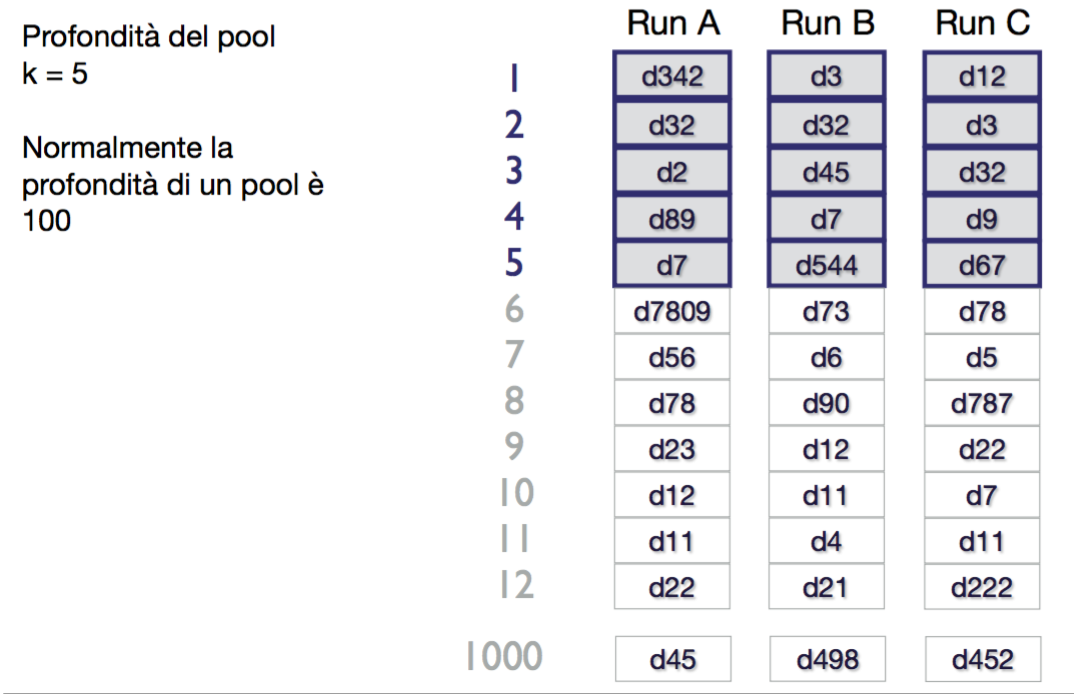
\includegraphics[width=0.5\textwidth]{images/l14-fig-2.png}
	\caption{Pool con profondità $k=5$}
\end{figure}

Vengono quindi utilizzati i documenti selezionati per creare un'insieme facendo l'unione, considerando una sola volta i documenti ripetuti (Figura \ref{fig:pool-union}) e solamente per questi documenti viene creato manualmente un giudizio di rilevanza.

\begin{figure}[htbp]
	\centering
	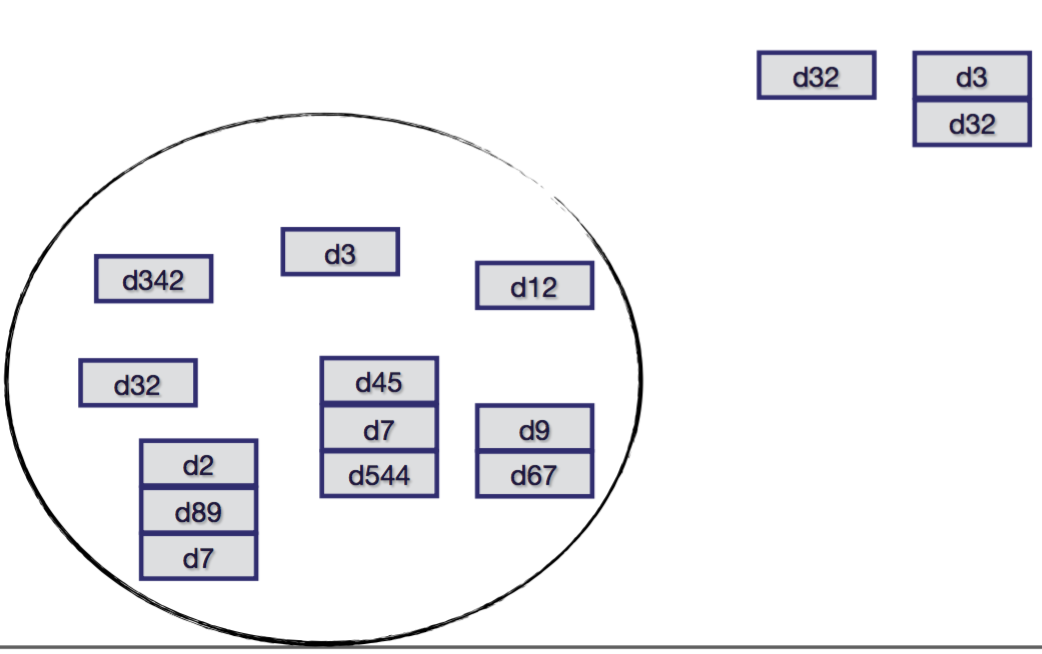
\includegraphics[width=0.45\textwidth]{images/l14-fig-3.png}
	\caption{Insieme dei documenti estratti dalle run e che compaiono nel pool}\label{fig:pool-union}
\end{figure}

Volendo si può prendere in considerazione da quanti sistemi un documento è stato considerato rilevante per creare una sorta di classificazione automatica, ma questo è un altro approccio che ha le stesse problematiche del campionamento casuale.

Tipicamente, se il giudizio è fatto in modo manuale, l'esperto non viene informato di quanti sistemi hanno valutato come rilevante il documento.

\begin{figure}[htbp]
	\centering
	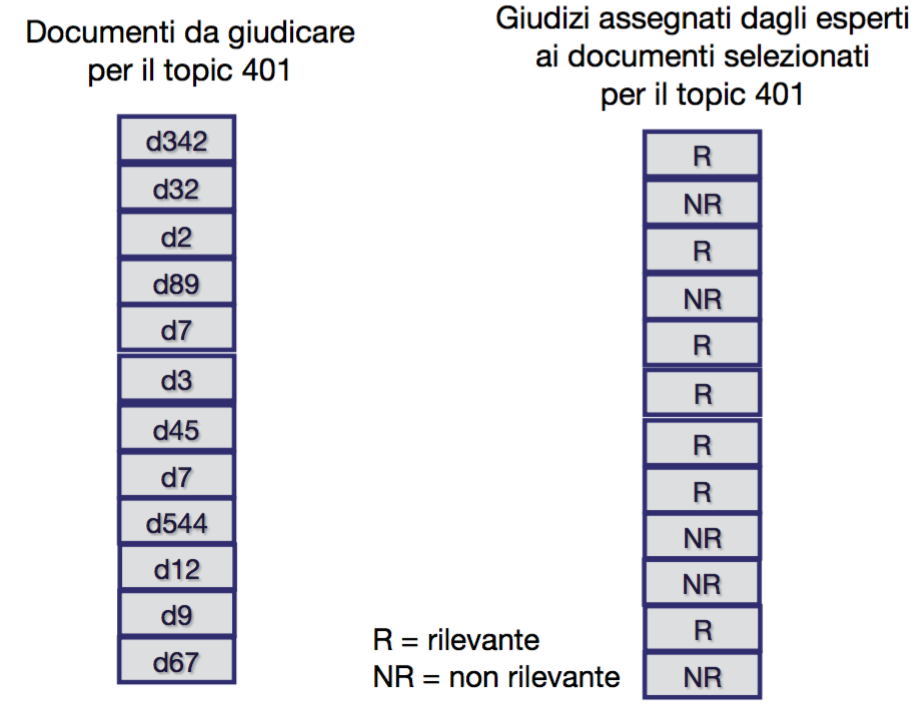
\includegraphics[width=0.45\textwidth]{images/l14-fig-4.png}
	\caption{Possibili giudizi di rilevanza dati dagli esperti ai documenti del pool}
\end{figure}

Tipicamente i documenti che non vengono giudicati sono marcati come non rilevanti. Ma non è sempre così, perché ci sono dei casi in cui vengono considerati come una via di mezzo.

Come profondità di pool, si ha che per TREC-[1-8] è 100, ma in altre collezioni è stato utilizzato 25, 30 o 125, tenendo a mente che minore è la profondità, minore è il pool.

\subsubsection{Completezza del pool}
\begin{center}
\textit{La valutazione di sistemi usando il pool e non un insieme completo di giudizi di rilevanza è stabile?}
\end{center}

Si è osservato, a seguito di uno studio su TREC-3, che i livelli di completezza sono \textbf{abbastanza} accettabili per \textbf{questo} tipo di valutazione.
Dallo studio è emerso che oltre la soglia dei 100, ci sono altri documenti rilevanti, ma non ne sono stati trovati abbastanza da influenzare in modo significativo (a livello statistico) la valutazione dei sistemi. Ovviamente questo è più probabile per i topic che hanno tanti documenti rilevanti.

\subsubsection{Robustezza del pool}

\begin{center}
\textit{Il pooling penalizza i sistemi le cui run non sono state incluse nel pool e/o che utilizzano metodologie molto differenti da quelle utilizzate dalla run considerate nel pool?}
\end{center}

Justin Zobel ha valutato ogni run usata per comporre il pool di TREC-5 usando in un primo momento i giudizi di rilevanza ufficiali di TREC (e quindi il pool) e successivamente un insieme di giudizi di rilevanza dove sono stati tolti (marcati non rilevanti) i documenti individuati solamente dalla run che stava valutando (leave-one-out).

Dallo studio è emerso che:

\begin{itemize}
	\item La qualità del pool (profondità e diversità delle run) non influenza in modo significativo la qualità della collezione di test.
	\item Ha verificato che le collezioni delle campagne di valutazione non sono \textit{biased} verso i sistemi le cui run non sono state considerate nel pool.
	\item Le \textit{prestazioni} delle run valutate con il pool originale erano più alte di quelle valutate con il pool ridotto mediamente dello $0.5\%$.
\end{itemize}

\section{Collezione di test e ground truth}

La tripla che identifica una collezione di test è

$$
\mathcal{C} = \{D, T, RJ (\text{o} \ P \ \text{da pool})\}
$$

\noindent Ma in generale parliamo di \textbf{ground truth} al posto dei pool e quindi la tripla diventa:

$$
\mathcal{C} = \{D, T, GT\}
$$

\noindent Sia $REL$ un insieme finito di \textbf{gradi di rilevanza} e sia $\preceq$ una relazione d'ordine totale su $REL$ tale che $(REL, \preceq)$ è un insieme totalmente ordinato (un insieme per il quale vale: riflessività, anti-simmetria, transitività e totalità).

Ad esempio $REL$ può essere:

$$
REL = \{nr, pr, fr, tr \}
$$

\noindent dove 
\begin{itemize}
	\item \textit{nr} = non rilevante;
	\item \textit{pr} = parzialmente rilevante;
	\item \textit{fr} = (\textit{failry})abbastanza rilevante;
	\item \textit{hr} = (\textit{highly})altamente rilevante.
\end{itemize}

\noindent A questo punto si può definire la relazione d'ordine

$$
nr \preceq pr \preceq fr \preceq hr
$$

La \textbf{ground truth} è quindi una funzione che dato un insieme finito di documenti $D$ e un insieme finito di topic $T$ associa alla coppia $(t,d)$ un valore di $REL$.

\begin{align*}
	GT : T \times D &\to REL \\
		(t,d) &\to rel
\end{align*}

\section{Misure con rilevanza binaria}

Una volta che è disponibile il pool per un dato topic è possibile giudicare (assess) ogni singola run rispetto al topic considerato.
Questa procedura prende il nome di \textbf{assessment}.

\begin{figure}[ht]
\centering
\begin{minipage}[b]{0.45\linewidth}
	\centering
  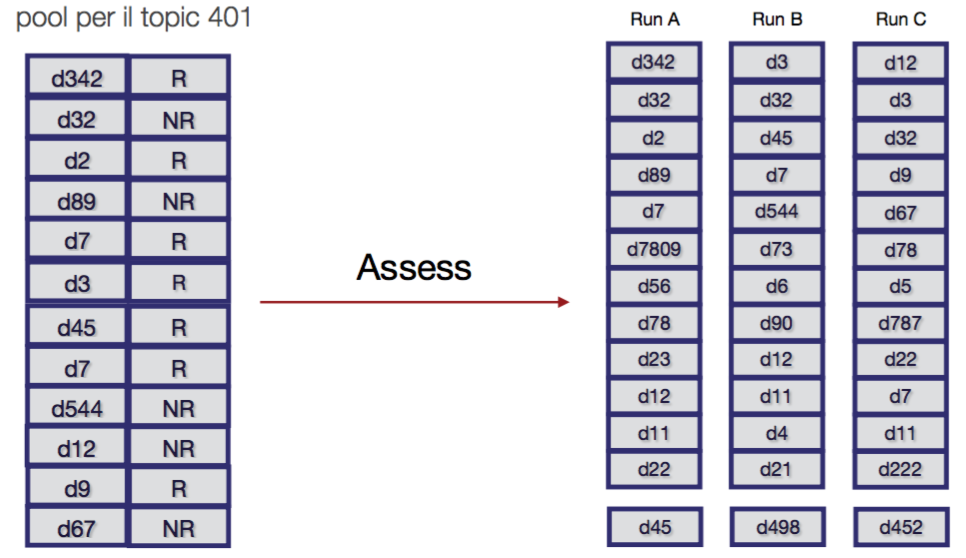
\includegraphics[width=0.95\textwidth]{images/l14-fig-5.png}
  \label{fig:minipage1}
  \caption{Assess relativi ai documenti}
\end{minipage}
\quad
\begin{minipage}[b]{0.45\linewidth}
	\centering
  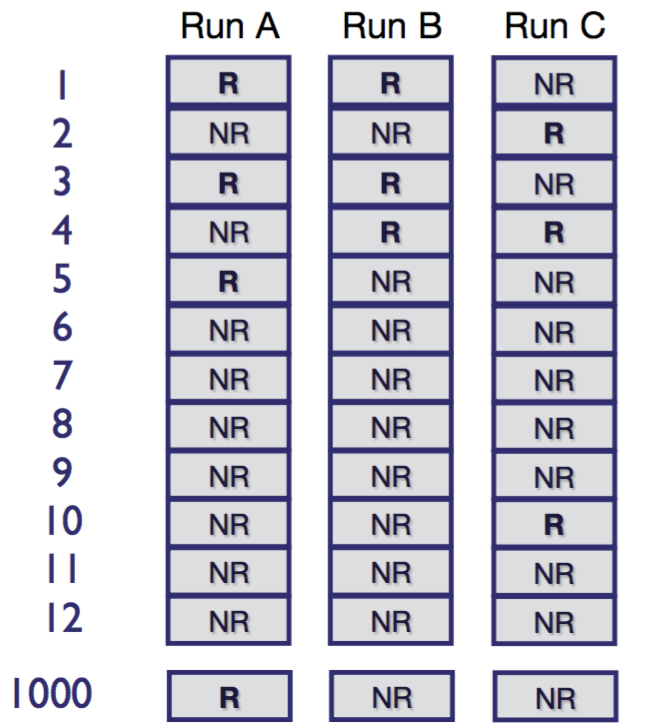
\includegraphics[width=0.6\textwidth]{images/l14-fig-6.png}
  \label{fig:minipage2}
  \caption{Da notare che per alcune run ci sono dei documenti rilevanti sotto i primi 5}
\end{minipage}
\end{figure}

\noindent ovvero le run precedenti diventano dei vettori con i giudizi di rilevanza.

Assegnare l'etichetta \textit{R} o \textit{NR} non è una grande scelta, si può quindi pensare di assegnare un valore numerico o un peso (\textbf{relevance weight}).

Si parla di \textbf{rilevanza binaria} se vengono utilizzati solo i pesi 0 o 1.
Se invece si hanno più possibili valori si parla di \textbf{multigraded relevance}.

\begin{figure}[htbp]
	\centering
	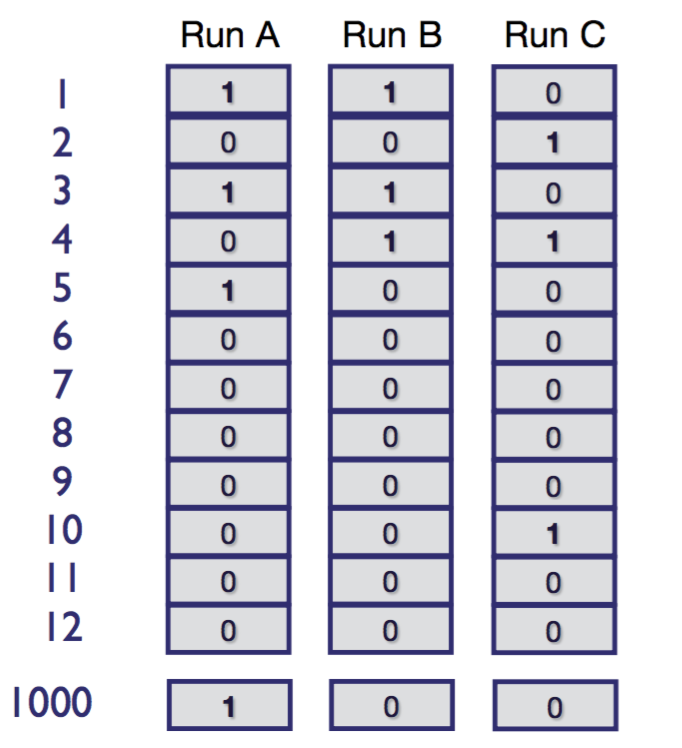
\includegraphics[width=0.4\textwidth]{images/l14-fig-7.png}
	\caption{Giudizi di rilevanza binari}
\end{figure}

Al fine della valutazione sono i vettori così ottenuti che ci interessano.

Per valutare una run, calcoliamo il \textbf{relevance score} $R(t) = \mathbf{r}_t$, una funzione:

\begin{align*}
	\hat{R} : T \times D^N &\to REL \\
	(t,\mathbf{r}_t) &\to \hat{\mathbf{r}_t} = (rel_1, rel_2, \ldots rel_N)
\end{align*}

\noindent dove $\hat{\mathbf{r}_t}[j] = GT(t, \mathbf{r}_t[j])$.

Ovvero è una funzione che associa ad ogni elemento di una run $\mathbf{r}_t$ il suo giudizio di rilevanza. 

Sia poi $W \subset \mathbf{Z}$ un insieme totalmente ordinato e finito di interi, $REL$ un insieme finito di gradi di rilevanza e sia $RW: REL \to W$ una funzione monotona che mappa ogni grado di rilevanza ($rel \in REL$) in un peso di rilevanza ($w \in W$), ovvero una funzione che associa ad ogni giudizio di rilevanza un valore numerico (peso).

\begin{figure}[htbp]
	\centering
	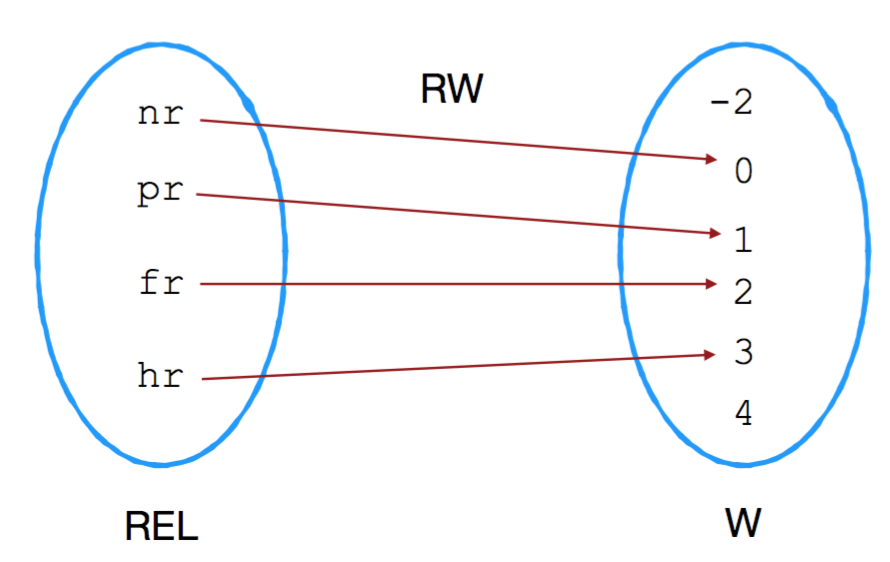
\includegraphics[width=0.4\textwidth]{images/l14-fig-8.png}
	\caption{Funzione $RW$}
\end{figure}

\noindent Quindi, data una run $R(t) = \mathbf{r}_t$ il suo \textbf{relevance weight} è una funzione

\begin{align*}
	\tilde{R}: T \times D^N &\to W^N \\
				(t, \mathbf{r}_t) &\to \tilde{\mathbf{r}}_t = (w_1, w_2, \ldots w_N)
\end{align*}

\noindent dove $\tilde{\mathbf{r}}_t[j] = RW(\hat{\mathbf{r}}_t[j])$

\begin{figure}[htbp]
	\centering
	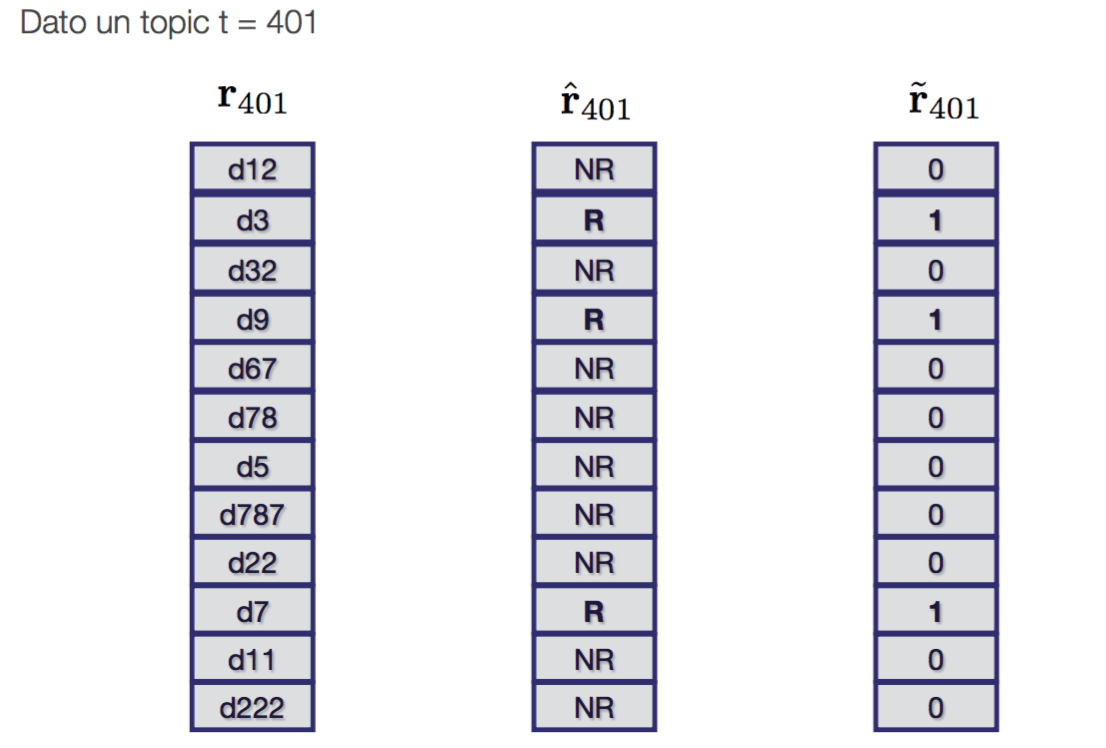
\includegraphics[width=0.6\textwidth]{images/l14-fig-9.png}
	\caption{Valutazione della run $\mathbf{r}_{401}$, prima con i giudizi di rilevanza e poi con la pesatura dei giudizi, in questo caso binari.}
\end{figure}
\FloatBarrier
\section{Precisione}

La \textit{Precision} misura quanti documenti rilevanti sono stati trovati, tra tutti quelli recuperati.

\begin{figure}[htbp]
	\centering
	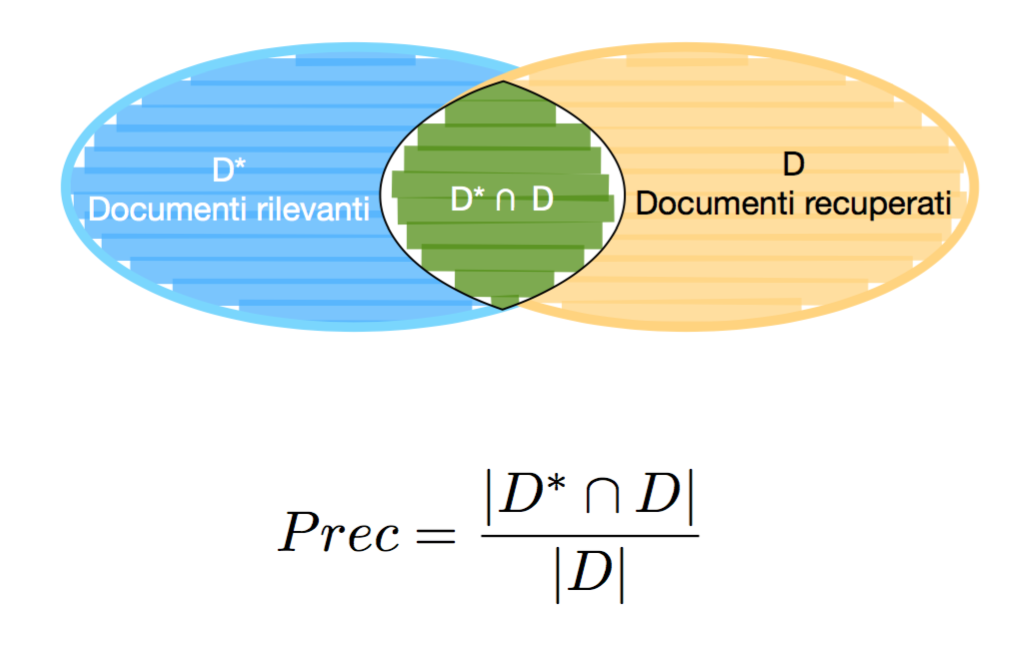
\includegraphics[width=0.4\textwidth]{images/l14-fig-10.png}
	\caption{Rappresentazione insiemistica della \textit{Precision}.}
\end{figure}
\FloatBarrier
\noindent La run migliore è quindi quella con il valore di precisione più alto. 
Ma non è detto che sia quella migliore per qualsiasi task, perché magari in ambito web è preferibile avere i primi elementi rilevanti, ovvero la run $X$, anche se è meno precisa.


\begin{figure}[htbp]
	\centering
	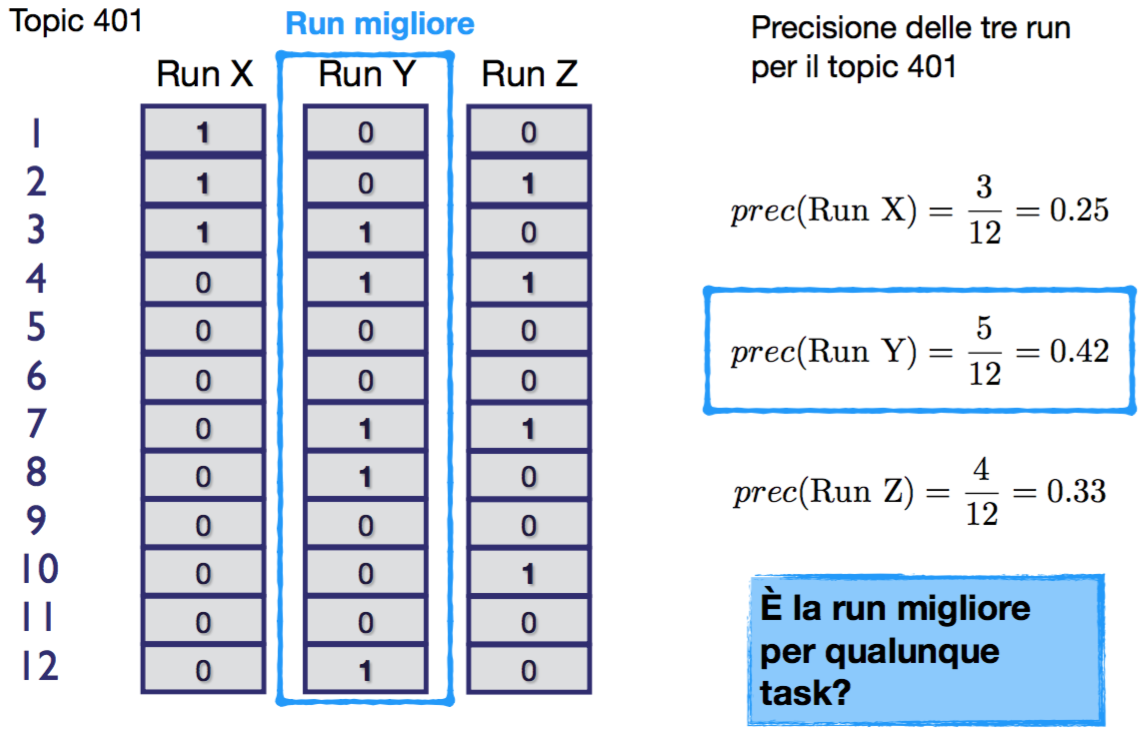
\includegraphics[width=0.55\textwidth]{images/l14-fig-11.png}
	\caption{Esempio di calcolo della \textit{Precision}. Vengono considerati solamente i primi 12 elementi per questioni pratiche.}
\end{figure}





